
\documentclass{beamer}

\usepackage{graphicx}
\usepackage{tabularx}
\usepackage[light]{FiraSans}
\usepackage[british]{datetime2}
\usetheme{default}
\setbeamertemplate{navigation symbols}{} % No navigation symbols
\definecolor{ntnu}{cmyk}{100,75,0,5}
\setbeamercolor{alerted text}{fg=ntnu}
\setbeamercolor{frame title}{fg=ntnu}
\setbeamercolor{title}{fg=ntnu}
\setbeamercolor{subtitle}{fg=ntnu}
\setbeamercovered{transparent}

\setbeamertemplate{itemize item}{\color{white}$\bullet$} % Comment this line for default bullet points (triangles)

\setbeamertemplate{footline}
{
\begin{tabularx}{\textwidth} {
	 >{\raggedright\arraybackslash}X 
  	 >{\centering\arraybackslash}X 
  	 >{\centering\arraybackslash}X 
  	 >{\centering\arraybackslash}X 
  	 >{\centering\arraybackslash}X 
  	 >{\centering\arraybackslash}X}
	
	\raisebox{-0.3cm}{
\includegraphics[width=2cm, keepaspectratio]{img/logo_ntnu_u-slagord.pdf}} &
	\insertshortauthor & 
	\insertshorttitle &
	\insertdate &
	\insertsection &
	$\big|$ \insertframenumber
\end{tabularx}
}

\makeatletter
\makeatother

%----------------------------------------------------------------------------------------
%	TITLE PAGE
%----------------------------------------------------------------------------------------

\title[Communal violence]{Precolonial states and communal violence}

\subtitle{}

\author[Wishman]{Marius Swane Wishman} 
\date{VIP presentation} 
\institute{ISS}

\begin{document}

\begin{frame}[plain]
\titlepage 
\centering

\includegraphics[width=5cm]{img/logo_ntnu_u-slagord.pdf} 
\end{frame}

\section{Precolonial states} 

\begin{frame}
\frametitle{Precolonial states} 
\end{frame}

\section{Communal violence}

\begin{frame}
\frametitle{First Section}
	
\end{frame}

\section{Relative peace in the absence of Leviathan}

\section{Leviathan}

\begin{frame}{Enter Leviathan}

	

\end{frame}

\section{}

\begin{frame}{The enduring effects of precolonial states}

	

\end{frame}

\section{Preliminary results}

\begin{frame}{Main results}

	\begin{figure}[htpb]
		\centering
		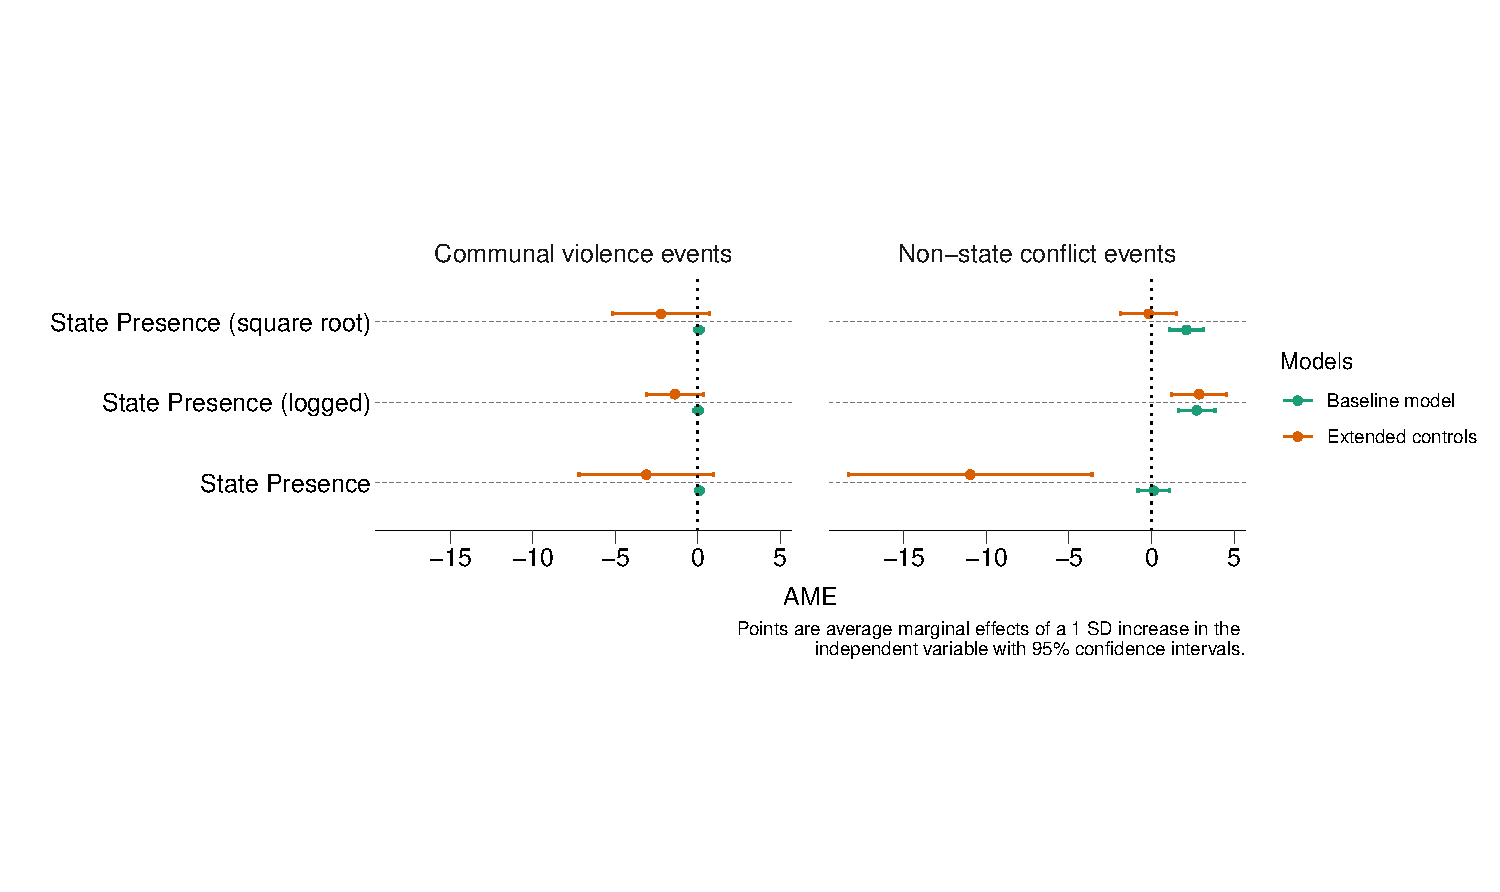
\includegraphics[width=0.8\linewidth]{../R/Output/CommunalViolenceMargins.pdf}
		\label{Margins}
	\end{figure}

\end{frame}

\section{What's next}

\begin{frame}{SIDE}

	

\end{frame}

\begin{frame}{Afrobarometer}

	

\end{frame}

\end{document}	
